\chapter{Solar Flares and the Forecasting Problem}
\label{ch:intro}

\section{Solar flares and space weather}

A solar flare is a sudden, localised release of magnetic energy in the Sun's
atmosphere, radiating across the electromagnetic spectrum on timescales of
minutes. Flares originate in \emph{active regions}~(ARs): concentrations of
strong, structured magnetic field that pierce the photosphere as sunspot
groups. The energy that powers a flare is not thermal but magnetic---it is
stored in electric currents that thread the coronal field and is liberated when
the field reconnects into a lower-energy configuration. The largest events are
frequently accompanied by coronal mass ejections, expelling magnetised plasma
into interplanetary space.

The practical importance of flares lies in their terrestrial impact, collectively
termed \emph{space weather}. Flare radiation and the energetic particles and
plasma that follow can disturb the ionosphere and disrupt high-frequency radio
communication and satellite navigation, induce currents in power grids, raise
radiation doses for astronauts and polar-route aircraft, and shorten the
operational lifetime of spacecraft. Because the radiative onset of a flare
arrives at Earth in a matter of minutes, useful mitigation depends on
\emph{forecasting}---estimating the probability of a significant event
\emph{before} it occurs, from the observable state of the source active region.

Flares are classified by their peak soft X-ray flux in the $1$--$8$~\AA{} band
measured by the GOES satellites, in a logarithmic scheme with classes A, B, C,
M and X. Operationally the threshold of concern is the M class and above:
$\geq$M events are energetic enough to drive the impacts listed above, yet rare
enough that reliable anticipation remains an open problem. Throughout this
thesis, ``a flare'' without further qualification refers to a $\geq$M event, and
forecasting is framed on the active-region scale using photospheric magnetic
data from the Helioseismic and Magnetic Imager (HMI) aboard the Solar Dynamics
Observatory (SDO). Figure~\ref{fig:goes} shows the classification scale and the
$\geq$M target regime.

% GOES soft X-ray flare classification scale (log flux bands A--X).
\begin{figure}[!htbp]
\centering
\begin{tikzpicture}[font=\small, >=Latex]
\def\w{2.2}   % band width
\foreach \i/\lab/\col/\flux in {
  0/A/gray!20/{$<10^{-7}$},
  1/B/blue!15/{$10^{-7}$},
  2/C/teal!20/{$10^{-6}$},
  3/M/orange!30/{$10^{-5}$},
  4/X/red!35/{$10^{-4}$}}{
  \fill[\col] (\i*\w,0) rectangle (\i*\w+\w,1);
  \draw (\i*\w,0) rectangle (\i*\w+\w,1);
  \node[font=\large\bfseries] at (\i*\w+\w/2,0.62) {\lab};
  \node[font=\scriptsize] at (\i*\w+\w/2,0.24) {\flux};
}
\node[font=\scriptsize] at (2.5*\w,-0.4) {peak $1$--$8$~\AA{} X-ray flux (W\,m$^{-2}$), logarithmic $\longrightarrow$};
% forecast-target bracket over M and X
\draw[thick,decorate,decoration={brace,amplitude=5pt}] (3*\w,1.15) -- (5*\w,1.15)
  node[midway,above=5pt,font=\small\bfseries]{forecast target: $\geq$M};
\end{tikzpicture}
\caption[GOES flare classes]{\textbf{The GOES soft X-ray flare classification.}
Flares are graded A--X by their peak $1$--$8$~\AA{} X-ray flux, each class a
factor of ten above the last. Operational concern---and the target of this
work---is the $\geq$M regime: energetic enough to drive space-weather impacts,
yet rare enough that reliable anticipation remains difficult.}
\label{fig:goes}
\end{figure}


\section{Why forecasting is hard}

The difficulty of flare forecasting is fundamental rather than merely technical.
Three properties conspire against it. First, the process is driven by the
\emph{coronal} magnetic field and its currents, whereas routine observations
resolve only the \emph{photospheric} field at the base of the atmosphere; the
quantity that matters must be inferred from a projection of it. Second, flaring
is governed by a threshold instability: an active region can store free energy
for days and release it in seconds, so the mapping from a slowly evolving
observable to a near-instantaneous event is weakly constrained. Third, $\geq$M
flares are \emph{rare}. In any large catalogue the flaring minority is
outnumbered by quiet examples by more than an order of magnitude, so a
forecaster is judged not on raw accuracy---trivially maximised by always
predicting ``quiet''---but on class-balanced skill scores such as the True Skill
Statistic (TSS), which reward correct anticipation of the rare positive class.

\section{The current forecasting landscape}
\label{sec:landscape}

Modern data-driven flare forecasting was catalysed by the availability of
uniform, machine-readable magnetic-field summaries of active regions. The
Space-weather HMI Active Region Patch (SHARP) product distils each AR's vector
magnetogram into a handful of scalar parameters---total unsigned flux, total
current helicity, twist, and related quantities. \citet{bobra2015} showed that a
support-vector machine trained on these SHARP scalars produces a competitive
$\geq$M forecaster, and established the SHARP feature vector as the de-facto
baseline against which later work is measured.

Two broad strands of deep learning followed. The first replaces hand-designed
scalars with features learned directly from the magnetogram \emph{image}:
\citet{huang2018} trained convolutional neural networks on line-of-sight
magnetograms, letting the network discover spatial precursors rather than
relying on pre-integrated summaries. The second exploits the \emph{temporal}
evolution of an active region: \citet{liu2019} fed sequences of SHARP parameter
vectors to a Long Short-Term Memory (LSTM) network, capturing the build-up of
free energy over the hours preceding an event, while operational systems such as
Deep Flare Net~\citep{nishizuka2018} combine engineered features with deep
architectures for daily probabilistic forecasts. The recurring lesson of this
literature is that both the \emph{spatial structure} of the field and its
\emph{temporal history} carry predictive information; the best systems try to
use both.

Running alongside this forecasting work is a strand of solar physics that seeks
a more physical descriptor of an active region's readiness to flare.
\citet{mactaggart2021} demonstrated that emerging active regions carry a
systematic magnetic \emph{winding}---a signed, topological measure of how field
lines wrap around one another---providing direct evidence that twisted flux
tubes create ARs. Magnetic winding flux is attractive precisely because it is
rooted in the field's topology rather than its raw strength, and it is the
central physical quantity of this thesis. Figure~\ref{fig:taxonomy} places these
strands, and the present work, in a single picture.

% Taxonomy of data-driven flare forecasting; where this thesis sits.
\begin{figure}[!htbp]
\centering
\begin{tikzpicture}[
  font=\small, >=Latex, node distance=6mm and 9mm,
  card/.style={draw, rounded corners=3pt, minimum height=13mm, text width=30mm,
               align=center, fill=black!4, inner sep=3pt},
  mine/.style={card, fill=green!14, very thick},
]
\node[card] (sharp) {\textbf{ML on SHARP scalars}\\\scriptsize SVM on integrated
  field parameters~\cite{bobra2015}};
\node[card, right=of sharp] (cnn) {\textbf{Deep spatial}\\\scriptsize CNN on
  magnetogram images~\cite{huang2018}};
\node[card, right=of cnn] (lstm) {\textbf{Deep temporal}\\\scriptsize LSTM on SHARP
  time series~\cite{liu2019,nishizuka2018}};
\node[card, below=14mm of sharp] (phys) {\textbf{Winding physics}\\\scriptsize signed
  topological precursor~\cite{mactaggart2021}};
\node[card, below=14mm of cnn] (scalar) {\textbf{Winding $\to$ scalars}\\\scriptsize
  integral + XGBoost~\cite{williams2026}};
\node[mine, below=14mm of lstm] (mine) {\textbf{Winding \emph{map} (this thesis)}\\
  \scriptsize 2D structure, spatiotemporal model};
\draw[->] (sharp) -- (cnn); \draw[->] (cnn) -- (lstm);
\draw[->] (phys) -- (scalar);
\draw[->, very thick, green!45!black] (scalar) -- (mine);
\draw[->, dashed] (lstm) -- (mine);
\draw[->, dashed] (phys) to[out=90,in=180] (sharp);
\end{tikzpicture}
\caption[Forecasting landscape]{\textbf{Where this thesis sits.} Data-driven
flare forecasting progressed from machine learning on integrated SHARP scalars
to deep spatial and deep temporal models. In parallel, magnetic winding emerged
as a physically motivated precursor, but existing work reduces the winding
\emph{map} to a single spatial integral, in which oppositely signed regions
cancel. This thesis instead feeds the two-dimensional winding map, with its
structure intact, to a spatiotemporal model.}
\label{fig:taxonomy}
\end{figure}


\section{Winding flux and the gap addressed by this thesis}

Magnetic winding flux is a \emph{signed} field defined pixel-by-pixel across an
active region: it is positive where field lines wind one way and negative where
they wind the other, and it is concentrated along polarity inversion lines,
where flares originate.

Formally, magnetic winding is a renormalisation of magnetic \emph{helicity}. The
relative helicity of a field $\mathbf{B}=\nabla\times\mathbf{A}$ is
$H=\int_V \mathbf{A}\cdot\mathbf{B}\,\mathrm{d}V$; the rate at which it is injected
through a photospheric plane $S$ can be written as a pairwise integral over
field-line footpoints \citep{prior2019},
\begin{equation}
  \frac{\mathrm{d}H}{\mathrm{d}t} = -\frac{1}{2\pi}\int_S\!\int_S
    \frac{\mathrm{d}\theta}{\mathrm{d}t}(\mathbf{x},\mathbf{y})\,
    B_z(\mathbf{x})\,B_z(\mathbf{y})\,\mathrm{d}^2x\,\mathrm{d}^2y,
  \label{eq:helicity}
\end{equation}
where $\theta(\mathbf{x},\mathbf{y})$ is the angle subtended by the two footpoints
and $\mathrm{d}\theta/\mathrm{d}t$ their relative rotation rate. Magnetic
\emph{winding} removes the flux weighting---each $B_z$ is replaced by its sign
$\sigma=\operatorname{sgn}(B_z)\in\{-1,0,+1\}$---so the measure depends on
field-line geometry alone \citep{mactaggart2020},
\begin{equation}
  \frac{\mathrm{d}L}{\mathrm{d}t} = -\frac{1}{2\pi}\int_S\!\int_S
    \frac{\mathrm{d}\theta}{\mathrm{d}t}(\mathbf{x},\mathbf{y})\,
    \sigma(\mathbf{x})\,\sigma(\mathbf{y})\,\mathrm{d}^2x\,\mathrm{d}^2y .
  \label{eq:winding}
\end{equation}
The integrand localises to a per-pixel \emph{winding-flux density}
\begin{equation}
  \dot{\mathcal{L}}(\mathbf{x}) = -\frac{1}{2\pi}\,\sigma(\mathbf{x})\!\int_S
    \frac{\mathrm{d}\theta}{\mathrm{d}t}(\mathbf{x},\mathbf{y})\,
    \sigma(\mathbf{y})\,\mathrm{d}^2y ,
  \label{eq:winddens}
\end{equation}
the signed map $\dot{\mathcal{L}}(\mathbf{x})$ that this thesis takes as its data:
at each point it is the net rotation of all other field lines about that point,
weighted only by their vertical sign. Comparing Eqs.~\eqref{eq:helicity} and
\eqref{eq:winding}, helicity is winding weighted by magnetic flux
($B_zB_z$ versus $\sigma\sigma$); winding therefore isolates the topology of the
near-horizontal field that helicity's flux weighting can mask, making it a
sensitive probe of the twisted, current-carrying field that precedes flaring.

Existing work that uses winding reduces the map to a
single number---its spatial integral---before forecasting. The most direct
example is recent: \citet{williams2026} derive scalar winding features from
active-region maps and feed them to gradient-boosted trees (XGBoost), obtaining
competitive flare-prediction skill and thereby confirming that winding carries
genuine predictive signal---yet the map is collapsed to a handful of numbers
before the classifier ever sees it. This integration is
convenient but lossy: because winding is signed, oppositely wound regions cancel
in the spatial mean, discarding exactly the localised, sign-resolved structure
that distinguishes a flare-productive configuration from a quiet one.
Figure~\ref{fig:windmap} makes the loss concrete: on a real active region the
magnitude of the spatial mean is roughly twenty times smaller than the spatial
standard deviation, so integrating to a scalar discards almost all of the
structure. To date, no study has fed the \emph{two-dimensional} winding-flux map,
with its spatial structure intact, to a deep model.

\begin{figure}[!htbp]
\centering
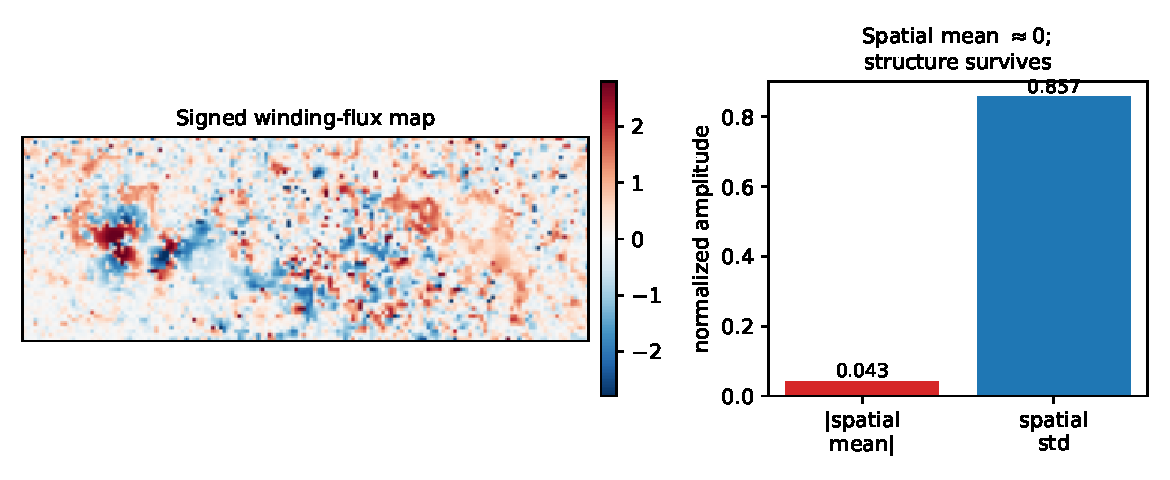
\includegraphics[width=0.92\textwidth]{figures/fig_winding_map.pdf}
\caption[Signed-mean cancellation]{\textbf{Why the spatial integral throws the
signal away.} Left: a signed winding-flux map of a real active region, with
oppositely wound (red/blue) regions. Right: the magnitude of the spatial mean is
only a small fraction of the spatial standard deviation---the positive and
negative winding very nearly cancel, so a single integrated scalar discards the
localised structure that the two-dimensional map retains.}
\label{fig:windmap}
\end{figure}

This thesis takes a first step into that gap. Rather than forecasting a flare
label directly, it asks a more basic question about the winding-flux field
itself: \emph{given a short history of winding-flux maps of an active region,
can a spatiotemporal deep model predict how the field evolves?} We treat this as
a \emph{proxy} task: a model that can anticipate the field's evolution must encode
the spatial structure and short-term dynamics of the winding field---
representations a downstream flare classifier could in principle reuse. Whether
such a representation actually improves flare classification is the question this
work sets up rather than settles. The vehicle for this study is
the Convolutional LSTM (ConvLSTM), a neural architecture that couples the spatial
inductive bias of convolution with the temporal memory of an LSTM, and is
therefore matched to the spatiotemporal nature of the data.

The remainder of the thesis is organised as follows. Chapter~\ref{ch:arch}
develops the technical architecture: the winding-flux data and its
representation, the ConvLSTM cell and the encoder--forecaster built from it, and
the training procedure. Chapter~\ref{ch:results} reports the forecasting
results, states plainly what the model does and does not achieve, and analyses
the outcome in light of the physical nature of the winding field---separating
genuine predictive skill from the persistence that a smoothly evolving field
affords for free.
